\chapter{Registration}

Image registration is a digital image processing technique that helps us align different images (for example, \gls{CT} and \gls{MRI} of the same scene.

ligning images from different time points or modalities (e.g., MRI and PET) requires interpolating pixel/voxel intensities when one image is transformed to match the other.

Useful for example for image averaging for increase the SNR.


\begin{center}
  \href{https://3dqlab.stanford.edu/image-registration/}{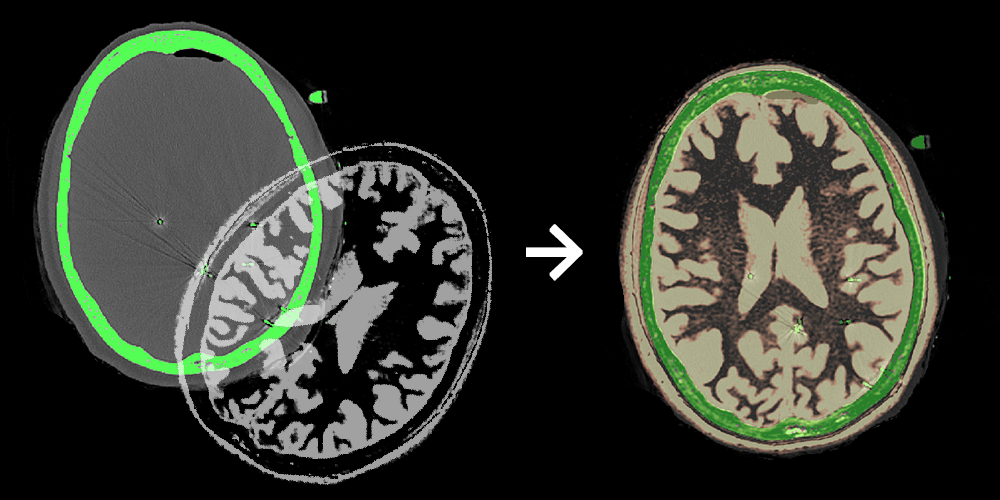
\includegraphics[width=12cm]{image_registration_example}}
\end{center}


\begin{verbatim}
# https://www.geeksforgeeks.org/python/image-registration-using-opencv-python/

import cv2
import numpy as np

# Open the image files.
img1_color = cv2.imread("align.jpg")  # Image to be aligned.
img2_color = cv2.imread("ref.jpg")    # Reference image.

# Convert to grayscale.
img1 = cv2.cvtColor(img1_color, cv2.COLOR_BGR2GRAY)
img2 = cv2.cvtColor(img2_color, cv2.COLOR_BGR2GRAY)
height, width = img2.shape

# Create ORB detector with 5000 features.
orb_detector = cv2.ORB_create(5000)

# Find keypoints and descriptors.
# The first arg is the image, second arg is the mask
#  (which is not required in this case).
kp1, d1 = orb_detector.detectAndCompute(img1, None)
kp2, d2 = orb_detector.detectAndCompute(img2, None)

# Match features between the two images.
# We create a Brute Force matcher with 
# Hamming distance as measurement mode.
matcher = cv2.BFMatcher(cv2.NORM_HAMMING, crossCheck = True)

# Match the two sets of descriptors.
matches = matcher.match(d1, d2)

# Sort matches on the basis of their Hamming distance.
matches.sort(key = lambda x: x.distance)

# Take the top 90 % matches forward.
matches = matches[:int(len(matches)*0.9)]
no_of_matches = len(matches)

# Define empty matrices of shape no_of_matches * 2.
p1 = np.zeros((no_of_matches, 2))
p2 = np.zeros((no_of_matches, 2))

for i in range(len(matches)):
  p1[i, :] = kp1[matches[i].queryIdx].pt
  p2[i, :] = kp2[matches[i].trainIdx].pt

# Find the homography matrix.
homography, mask = cv2.findHomography(p1, p2, cv2.RANSAC)

# Use this matrix to transform the
# colored image wrt the reference image.
transformed_img = cv2.warpPerspective(img1_color,
                    homography, (width, height))

# Save the output.
cv2.imwrite('output.jpg', transformed_img)

\end{verbatim}